\documentclass{article}
\usepackage{spikey}
\usepackage{amsmath}
\usepackage{mathrsfs}
\usepackage{amssymb}
\usepackage{soul}
\usepackage{float}
\usepackage{graphicx}
\usepackage{hyperref}
\usepackage{xcolor}
\usepackage{chngcntr}
\usepackage{centernot}
\usepackage[shortlabels]{enumitem}
\usepackage[margin=1truein]{geometry}
\usepackage{tkz-graph}
\usepackage{dsfont}

\counterwithin{equation}{section}
\counterwithin{figure}{section}

\usepackage[
    type={CC},
    modifier={by-nc},
    version={4.0},
]{doclicense}

\title{MAT395 Independent Reading in Mathematical Economics\\ \small Individual Decision Making, Market Equilibrium, Market Failure, and Other Topics.}
\date{\today}
\author{Tianyu Du}
\begin{document}
	\maketitle
	\doclicenseThis
	\begin{itemize}
		\item GitHub: \url{https://github.com/TianyuDu/Spikey_UofT_Notes}
		\item Website: \url{TianyuDu.com/notes}
	\end{itemize}
	\tableofcontents
	\newpage
	
	\section{Chapter 1. Preference and Choice}
	\subsection{Preference Relations}
	
		\begin{definition} \quad
			\begin{enumerate}[(i)]
				\item The \textbf{strict preference} relation, $\succ$, is defined by
					\begin{equation}
						x \succ y \iff x \pref y \land \neg (y \pref x)
					\end{equation}
				\item The \textbf{indifference} relation, $\sim$, is defined by
					\begin{equation}
						x \sim y \iff x \pref y \land y \pref x
					\end{equation}
			\end{enumerate}
		\end{definition}
	
		\begin{definition}[1.B.1]
			The preference relation $\pref$ is \textbf{rational} if it possesses the following two properties
			\begin{enumerate}[(i)]
				\item \emph{Completeness} 
					\begin{equation}
						\forall x, y \in X,\ x \pref y \lor y \pref x
					\end{equation}
				\item \emph{Transitivity}
					\begin{equation}
						\forall x, y, z \in X,\ x \pref y \land y \pref z \implies x \pref z
					\end{equation}
			\end{enumerate}
		\end{definition}
	
		\begin{proposition}[1.B.1]
			If $\pref$ is rational, then
			\begin{enumerate}[(i)]
				\item $\succ$ is both \textbf{reflexive} ($\neg\ x \succ x$) and \textbf{transitive} ($x \succ y \land y \succ z \implies x \succ z$);
				\item $\sim$ is both \textbf{reflexive} and \textbf{transitive};
				\item $x \succ y \pref z \implies x \succ z$.
			\end{enumerate}
		\end{proposition}
		
		\begin{example}
			Typical scenarios when transitivity of preference is violated:
			\begin{enumerate}[(i)]
				\item \emph{Just perceptible differences};
				\item \emph{Framing problem};
				\item \emph{Observed preference might from the result of the interaction of several more primitive rational preferences (Condorcet paradox)};
				\item \emph{Change of tastes}.
			\end{enumerate}
		\end{example}
		
		\begin{definition}[1.B.2]
			A function $u: X \to \R$ is a \textbf{utility function representing preference relation} $\pref$ if
			\begin{equation}
				\forall x, y \in X,\ x \pref y \iff u(x) \geq u(y)
			\end{equation}
		\end{definition}
		
		\begin{proposition}[1.B.2]
			If a preference relation $\pref$ can be represented by a utility function, then $\pref$ is rational.
		\end{proposition}
	
	\subsection{Choice Rules}
		\begin{definition}
			A \textbf{choice structure}, $(\mathscr{B}, C(\cdot))$, is a tuple consists of
			\begin{enumerate}[(i)]
				\item The collection of \textbf{budget sets} $\mathscr{B}$, which is a set of nonempty subsets of $X$.
				\item The \textbf{choice rule}, $C(B) \subset B$, is a \emph{correspondence} for every $B \subset \mathscr{B}$ denotes the individual's choice from among the alternatives in $B$. If $C(B)$ is not a singleton, it can be interpreted as the \emph{acceptable alternatives} in $B$, which the individual would actually chosen if the decision-making process is run repeatedly. 
			\end{enumerate}
		\end{definition}
		
		\begin{definition}[1.C.1]
			The choice structure $(\mathscr{B}, C(\cdot))$ satisfies the \textbf{weak axiom of revealed preference} if
			\begin{equation}
				\Big(\underbrace{
					\exists B \in \mathscr{B}\ s.t.\ x, y \in B \land x \in C(B)
					}_{\tx{$x \pref* y$ revealed.}}
				\Big)
				\implies 
				\Big(
					\forall B' \in \mathscr{B}\ s.t.\ x, y \in B',\ y \in C(B') \implies x \in C(B')
				\Big)
			\end{equation}
		\end{definition}
		
		\begin{definition}
			Given a choice structure $(\mathscr{B}, C(\cdot))$, the \textbf{revealed preference relation} $\pref^*$ is defined as
			\begin{equation}
				x \pref^* y \iff \exists B \in \mathscr{B}\ s.t.\ x, y \in B \land x \in C(B)
			\end{equation}
		\end{definition}
		
		\begin{remark}[Interpretation on the definition of WARP]
			If $x$ is \emph{revealed} at least as good as $y$, then $y$ cannot be revealed preferred to $x$.
		\end{remark}
	
	\subsection{The Relationship between Preference Relations and Choice Rules}
		\begin{definition}
			Given \ul{rational} preference relation $\pref$ on $X$, the \textbf{preference-maximizing choice rule} is defined as 
			\begin{equation}
				C^*(B, \pref) := \{x \in B: x \pref y\ \forall y \in B\}\ \forall B \in \mathscr{B}
			\end{equation}
			We say the \ul{rational} preference relation \textbf{generates} the choice structure $(\mathscr{B}, C^*(\cdot, \pref))$.
		\end{definition}
		
		\begin{assumption}
			Assume $C^*(B, \pref) \neq \varnothing$ for all $B \in \mathscr{B}$.
		\end{assumption}
		
		\begin{proposition}[1.D.1 (\hl{Rational $\to$ WARP})]
			Suppose that $\pref$ is a \ul{rational} preference relation. Then the choice structure generated by $\pref$, $(\mathscr{B}, C^*(\cdot, \pref))$, satisfies the weak axiom.
		\end{proposition}
		
		\begin{definition}[1.D.1]
			Given choice structure $(\mathscr{B}, C(\cdot))$, we say that the \ul{rational preference relation $\pref$ \textbf{rationalizes} $C(\cdot)$ relative to $\mathscr{B}$} if
			\begin{equation}
				C(B) = C^*(B, \pref)\ \forall B \in \mathscr{B}
			\end{equation}
			That is, \emph{$\pref$ generates the choice structure $(\mathscr{B}, C(\cdot))$}.
		\end{definition}
		
		\begin{remark}
			In general, for a given choice structure $(\mathscr{B}, C(\cdot))$, there may be more than one rational preference relation $\pref$ rationalizing it.
		\end{remark}
		
		\begin{proposition}[1.D.2 (\hl{WARP $\to$ Rational})]
			If $(\mathscr{B}, C(\cdot))$ is a choice structure such that
			\begin{enumerate}[(i)]
				\item The weak axiom is satisfied;
				\item $\mathscr{B}$ includes all subsets of $X$ up to three elements.
			\end{enumerate}
			Then there is a rational preference relation $\pref$ that rationalizes $C(\cdot)$ relative to $\mathscr{B}$.
		\end{proposition}
	
	\section{Chapter 2. Consumer Choice}
		\subsection{Commodities}
			\begin{definition}
				Assume the number of \textbf{commodities} is finite and equal to $L$. In general, a \textbf{commodity vector} or \textbf{commodity bundle} is an element in a \textbf{commodity space}, typically $\R^L$.
				\begin{equation}
					\vex := \begin{bmatrix}
						x_1 \\ \vdots \\ x_L
					\end{bmatrix} \in \R^L
				\end{equation}
 			\end{definition}
 			
 			\begin{remark}[Time Aggregation]
 				The time/location of commodity matters in some scenarios, and can be built into the definition of a commodity.
 			\end{remark}
 			
 			\begin{remark}
 				We should also note that in some contexts it becomes convenient, and even necessary, to expand the set of commodities to include goods and services that may potentially be available for purchase but are not actually so and even some that may be available by means other than market exchange.
 			\end{remark}
 		
 		\subsection{The Consumption Set}
 			\begin{definition}
 				The \textbf{consumption set} is a subset of the commodity space $\R^L$, denoted by $X \subset \R^L$, whose elements are the consumption bundles that the individual can conceivably consume given the physical constraints imposed by his environment.
 			\end{definition}
 			
 			\begin{assumption}
 				For simplicity, we assume the consumption set to be $\R_+^L$, which is \emph{convex}.
 				\begin{equation}
 					X := \R_+^L = \{\vex \in \R^L: x_{\ell} \geq 0,\ \forall \ell \in [L]\}
 				\end{equation}
 			\end{assumption}
 			
 		\subsection{Competitive Budgets}
 			\begin{definition}
 				A \textbf{price vector} is defined as
 				\begin{equation}
 					\vep := \begin{bmatrix} p_1 \\ \vdots \\ p_L \end{bmatrix} \in \R^L
 				\end{equation}
 				For simplicity, here we always assume 
 				\begin{enumerate}[(i)]
 					\item \emph{Positive price}: $\vep \gg \ve{0}$;
 					\item \emph{Price-taking assumption}: $\vep$ is beyond the influence of the consumer.
 				\end{enumerate}
 			\end{definition}
 			
 			\begin{definition}[2.D.1]
 				The \textbf{Walrasian}, or \textbf{competitive budget set} is defined as
 				\begin{equation}
 					B_{\vep, w} := \{
 						\vex \in \R^L_+: \vep \cdot \vex \leq w
 					\}
 				\end{equation}
 				where $w$ is the \emph{wealth} of consumer, and assumed to be positive.
 			\end{definition}
 			
 			\begin{definition}
 				The \textbf{consumer's problem} is choosing a consumption bundle $\vex \in B_{\vep, w}$, for each given $(\vep, w) \in \R^L_{++}$.
 			\end{definition}
 			
 			\begin{definition}
 				The set $\{\vex \in \R^L_+: \vep \cdot \vex = w\}$ is called the \textbf{budget hyperplane}.
 			\end{definition}
 			
 			\begin{proposition}
 				The price vector $\vep$ is orthogonal to the budget hyperplane.
 			\end{proposition}
 			
 			\begin{proposition}
 				The Walrasian budget set $B_{\vep, w}$ is a \emph{convex} set.
 			\end{proposition}
 		
 		\subsection{Demand Functions and Comparative Statics}
 			\begin{definition}
 				The consumer's \textbf{Walrasian demand correspondence} $x(\vep, w): \R_{++}^{L+1} \rightrightarrows \R_+^L$ assigns a \emph{set} of chosen consumption bundles for each price-wealth pair $(\vep, w)$. When $x(\vep, w)$ is single-valued, we refer to it as a \textbf{demand function}
 				\begin{equation}
 					\vex(\vep, w) = 
 					\begin{bmatrix}
 						x_1(\vep, w) \\
 						x_2(\vep, w) \\
 						\vdots \\
 						x_L(\vep, w)
 					\end{bmatrix}
 				\end{equation}
 			\end{definition}
 			
 			\begin{definition}[2.E.1]
 				The Walrasian demand correspondence $x(\vep, w): \R_{++}^{L+1} \rightrightarrows \R_+^L$ is \textbf{homogenous of degree zero} if 
 				\begin{equation}
 					x(\alpha \vep, \alpha w) = x(\vep, w)\ \forall (\vep, w, \alpha) \in \R_{++}^{L+2}
 				\end{equation}
 				Also note that
 				\begin{equation}
 					B_{\vep, w} = B_{\alpha \vep, \alpha w}\ \forall (\vep, w, \alpha) \in \R_{++}^{L+2}
 				\end{equation}
 			\end{definition}
 			
 			\begin{definition}[2.E.2]
 				The Walrasian demand correspondence $x(\vep, w)$ satisfies \textbf{Walras' law} if
 				\begin{equation}
 					\forall (\vep, w) \gg \ve{0},\ \forall \vex \in x(\vep, w),\ \vep \cdot \vex = w
 				\end{equation}
 			\end{definition}
 			
 			\begin{assumption}
 				For simplicity, we assume $x(\vep, w)$ is always \emph{single-valued, continuous and differentiable}.
 			\end{assumption}
 			
 			\begin{proposition}
 				The \textbf{family of Walrasian budget sets} defined as
 				\begin{equation}
 					\mathscr{B}^{\mathscr{W}} := \{B_{\vep, w}: {\vep, w} \gg \ve{0}\}
 				\end{equation}
 				altogether with Walrasian demand homogeneous to degree zero forms a \emph{choice structure}
 				\begin{equation}
 					(\mathscr{B}^{\mathscr{W}}, x(\cdot))
 				\end{equation} 
 			\end{proposition}
 		
 			\begin{definition}
 				For fixed prices $\overline{\vep} \in \R_{++}^L$, the function of wealth $\vex(\overline{\vep}, w)$ is called consumer's \textbf{Engel function}. Its image in $\R^L_+$,
 				\begin{equation}
 					E_{\overline{\vep}} := \{\vex(\overline{\vep}, w): w \in \R_{++}\} \subset \R^L_+
 				\end{equation}
 				is defined as the \textbf{wealth expansion path}.
 			\end{definition}
 			
 			\begin{definition}
 				Given $(\vep, w)$, the \textbf{wealth effect} is defined as
 				\begin{equation}
 					D_w \vex(\vep, w) 
 					= \begin{bmatrix}
 						\pd{x_1(\vep, w)}{w} \\
 						\pd{x_2(\vep, w)}{w} \\
 						\vdots \\
 						\pd{x_L(\vep, w)}{w}
 					\end{bmatrix} \in \R^L
 				\end{equation}
 				For the $\ell$-th commodity, it's called \textbf{normal} at $(\vep, w)$ if $\pd{x_{\ell}(\vep, w)}{w} \geq 0$, and \textbf{inferior} otherwise. And the $\ell$-th commodity is normal/inferior if its normal/inferior every where in $\R_{++}^{L+1}$. 
 			\end{definition}
 			
 			\begin{definition}
 				The \textbf{offer curve} is defined as the locus
 				\begin{equation}
 					\{\vex(\vep, w): p_j > 0\}
 				\end{equation}
 				for any chosen $j$.
 			\end{definition}
 			
 			\begin{definition}
 				Good $\ell$ is said to be a \textbf{Giffen good} at $(\vep, w)$ if
 				\begin{equation}
 					\pd{x_\ell(\vep, w)}{p_\ell} > 0
 				\end{equation}
 			\end{definition}
 			
 			\begin{definition}
 				The \textbf{price effects} at $(\vep, w)$ is defined as
 				\begin{equation}
 					D_{\vep} (\vep, w) = 
 					\begin{bmatrix}
 						\pd{x_1(\vep, w)}{p_1} & \cdots & \pd{x_1(\vep, w)}{p_L} \\
 						& \ddots & \\
 						\pd{x_L(\vep, w)}{p_1} & \cdots & \pd{x_L(\vep, w)}{p_L}
 					\end{bmatrix}
 				\end{equation}
 			\end{definition}
 			
 			\begin{proposition}[2.E.1]
 				If the Walrasian demand function $x(\vep, w)$ is homogenous of degree zero, then for all $\vep$ and $w$, then
 				\begin{equation}
 					\sum_{k=1}^{L} \frac{\partial x_{\ell}(\vep, w)}{\partial p_{k}} p_{k}+\frac{\partial x_{\ell}(\vep, w)}{\partial w} w=0 \text { for } \ell=1, \ldots, L
 				\end{equation}
 				Equivalently,
 				\begin{equation}
 					D_{\vep} \vex (\vep, w)\ \vep + D_w \vex(\vep, w)\ w = \ve{0}
 				\end{equation}
 				\begin{proof}
 					Apply \emph{Euler's theorem} on homogenous functions to each component $x_\ell$.
 					\begin{gather}
 						\underbrace{D_{(\vep, w)} \vex(\vep, w)}_{L \times (L+1)} \cdot \underbrace{(\vep, w)}_{(L+1) \times 1} = 0\ \vex(\vep, w) = \ve{0} \\
 						\implies [\underbrace{D_{\vep} (\vep, w)}_{L \times L} | \underbrace{D_w \vex(\vep, w)}_{L \times 1}] \cdot (\vep, w) = D_{\vep} (\vep, w)\ \vep + D_w \vex(\vep, w)\ w = \ve{0}
 					\end{gather}
 				\end{proof}
 			\end{proposition}
 			
 			\begin{definition}
 				The \textbf{elasticities of demand $\ell$ with respect to price $k$ and wealth} is defined as 
 				\begin{gather}
 					\varepsilon_{\ell, k} (\vep, w) := \pd{x_\ell (\vep, w)}{p_k} \frac{p_l}{x_\ell (\vep, w)}\\
 					\varepsilon_{\ell, w} (\vep, w) := \pd{x_\ell (\vep, w)}{w} \frac{w}{x_\ell (\vep, w)}
 				\end{gather}
 			\end{definition}
 			
  			\begin{corollary}
  				Dividing both sides of the equality in proposition (2.E.1) by $x_{\ell}$ gives
 				\begin{equation}
 					\sum_{k=1}^L \varepsilon_{\ell, k}(\vep, w) + \varepsilon_{\ell, w}(\vep, w) = 0\ \forall \ell \in \{1, \ldots, L\}
 				\end{equation}
 			\end{corollary}
 			
 			\begin{proposition}[2.E.2 Cournot Aggregation]
 				If the Walrasian demand function $x(\vep, w)$ satisfies \emph{Walras' law}, then for every $(\vep, w)$,
 				\begin{equation}
 					\sum_{\ell=1}^{L} p_{\ell} \frac{\partial x_{\ell}(\vep, w)}{\partial p_{k}}+x_{k}(\vep, w)= 0 \quad \text { for } k=1, \ldots, L
 				\end{equation}
 				Equivalently,
 				\begin{equation}
 					\vep^T D_{\vep} \vex (\vep, w) + \vex(\vep, w)^T = \ve{0}^T
 				\end{equation}
 				\begin{proof}
 					Differentiate both sides of Walras' law identity $\vep^T \vex = w$ with respect to $\vep$.
 				\end{proof}
 			\end{proposition}
 			
 			\begin{proposition}[2.E.3. Engel Aggregation]
 				If the Walrasian demand function $x(\vep, w)$ satisfies \emph{Walras' law}, then for every $(\vep, w)$,
 				\begin{equation}
 					\sum_{\ell=1}^{L} p_{\ell} \frac{\partial x_{\ell}(\vep, w)}{\partial w}=1
 				\end{equation}
 				or equivalently
 				\begin{equation}
 					\vep \cdot D_{w} x(\vep, w) = 1
 				\end{equation}
 				\begin{proof}
 					Differentiate both sides of Walras' law identity $\vep^T \vex = w$ with respect to $w$.
 				\end{proof}
 			\end{proposition}
 		
 			\begin{proposition}[Exer. 2.E.2]
 				\begin{gather}
 					\sum_{\ell=1}^{L} b_{\ell}(\vep, w) \varepsilon_{\ell k}(\vep, w)+b_{k}(\vep, w)=0
 				\end{gather}
 				and
 				\begin{gather}
 					\sum_{\ell=1}^{L} b_{\ell}(\vep, w) \varepsilon_{\ell w}(\vep, w)=1
 				\end{gather}
 				where $b_\ell := \frac{x_\ell p_\ell}{w}$ is defined to be the portion of wealth spent on commodity $\ell$.
 			\end{proposition}
 			
 		\subsection{The Weak Axiom of Revealed Preference and the Law of Demand}
 			\begin{assumption}
 				In the section, we assume $\vex(\vep, w)$ is 
 				\begin{enumerate}[(i)]
 					\item Single-valued;
 					\item homogeneous to degree zero;
 					\item satisfies Walras' law.
 				\end{enumerate}
 			\end{assumption}
 			
 			\begin{definition}[2.F.1]
 				The Walrasian demand function $\vex(\vep, w)$ satisfies the \textbf{weak axiom of revealed preference} if for every two $(\vep, w), (\vep', w') \in \R_{++}^{L+1}$,
 				\begin{gather}
 					\underbrace{\vep \cdot \vex(\vep', w') \leq w
 					\land \vex(\vep, w) \neq \vex(\vep', w')}_{\tx{revealed: } \vex(\vep, w) \succ^* \vex(\vep', w')}
 					\implies \vep' \cdot \vex(\vep, w) > w'
 				\end{gather}
 				Equivalently,
 				\begin{equation}
 					\vex(\vep', w') \in B_{\vep, w} \land \vex(\vep', w') \centernot \in C(B_{\vep, w}) \implies \vex(\vep, w) \centernot \in C(B_{\vep', w'})
 				\end{equation}
 			\end{definition}
 			
 			\begin{corollary}[Equivalent Definition ]
 				The weak axiom says, given our assumptions and $\vex(\vep_1, w_1) \neq \vex(\vep_2, w_2)$, we \ul{cannot} have both 
 				\begin{equation}
 					\vex(\vep_1, w_1) \in B_{\vep_2, w_2} \land \vex(\vep_2, w_2) \in B_{\vep_1, w_1}
 				\end{equation}
 			\end{corollary}
 			
 			\begin{definition}
 				A price change $\Delta \vep$ is a \textbf{Slutsky compensated price change} if the consumer is given a \textbf{Slutsky wealth compensation} with amount
 				\begin{equation}
 					\Delta w = \Delta \vep \cdot \vex(\vep, w)
 				\end{equation}
 				such that the consumer's initial consumption is just affordable at the new price.
 			\end{definition}
 			
 			\begin{proposition}[2.F.1]
 				Suppose that the Walrasian demand function $\vex(\vep', w')$ is homogenous of degree zero and satisfies Walras' law. Then $\vex(\vep', w')$ satisfies the weak axiom \ul{if and only if} the following property holds: \\
 				For any \emph{compensated price change} from $(\vep, w)$ to $(\vep', w' := \vep' \cdot \vex(\vep, w))$,
 				\begin{equation}
 					\Delta \vep \cdot \Delta \vex \leq 0
 				\end{equation}
 				with strict inequality whenever $\vex(\vep, w) \neq \vex(\vep', w')$.
 			\end{proposition}
 			
 			\begin{corollary}[Compensated Law of Demand]
 				$\Delta \vep \cdot \Delta \vex \leq 0$ says demand and price move in opposite directions, \emph{under Slutsky compensation}.
 			\end{corollary}
 			
 			\begin{definition}
 				At infinitesimal price change, the Slutsky compensation can be written as 
 				\begin{equation}
 					dw = \vex(\vep, w) \cdot d\vep
 				\end{equation}
 				and the compensated law of demand becomes
 				\begin{equation}
 					d\vep \cdot d\vex \leq 0
 				\end{equation}
 				Then the total derivative of $\vex$ is 
 				\begin{align}
 					d\vex &= D_\vep\vex(\vep, w)\ d\vep + D_w \vex(\vep, w)\ dw \\
 					&= D_\vep\vex(\vep, w)\ d\vep + D_w \vex (\vep, w)\ [\vex(\vep, w) \cdot d\vep] \\
 					&= [\underbrace{D_\vep\vex(\vep, w)}_{L \times L} + \underbrace{D_w \vex (\vep, w)}_{L \times 1} \underbrace{\vex(\vep, w)^T}_{1 \times L}] d\vep \\
 					&\implies d\vep^T 
 					\underbrace{[D_\vep\vex(\vep, w) + D_w \vex (\vep, w) \vex(\vep, w)^T]}_{L \times L} d\vep \leq 0
 				\end{align}
 				and the \textbf{Slutsky/substitution matrix} is defined as
 				\begin{gather}
 					S(\vep, w) := [D_\vep\vex(\vep, w) + D_w \vex (\vep, w) \vex(\vep, w)^T] \\
 					s_{\ell k} = \underbrace{\pd{x_\ell(\vep, w)}{p_k}}_{\tx{total effect}} + \underbrace{\pd{x_\ell(\vep, w)}{w} x_k (p, w)}_{\tx{wealth effect}}
 				\end{gather}
 				where $s_{\ell k}$ is the \textbf{substitution effect}.
 			\end{definition}
 			
 			\begin{remark}
 				The above identity (Slutsky equation) suggests the total impact of price change in $p_k$ on demand for $x_{\ell}$ can be decomposed into two portions, substitution effect and income effect.
 			\end{remark}
 			
  			\begin{corollary}[Slutsky Equation]
 				\begin{equation}
 					\frac{\partial x_{i}(\mathbf{p}, w)}{\partial p_{j}}=\frac{\partial h_{i}(\mathbf{p}, u)}{\partial p_{j}}-\frac{\partial x_{i}(\mathbf{p}, w)}{\partial w} x_{j}(\mathbf{p}, w)
 				\end{equation}
 			\end{corollary}
 			
 			\begin{remark}
 				Consider the scenario when only $p_k$ changes, with Slutsky compensation, consumer's wealth changes by $dw = x_k(\vep, w) dp_k$. So the wealth effect on $x_\ell$ is $\pd{x_\ell}{w} dw = \pd{x_\ell}{w} x_k(\vep, w) dp_k$.
 			\end{remark}
 			
 			\begin{proposition}[2.F.2]
 				If a differentiable Walrasian demand function $\vex(\vep, w)$ satisfies Walras' law, homogeneity of degree zero, and the weak axiom, then at any $(\vep, w)$, the Slutsky matrix $S(\vep, w)$ is negative semi-definite.
 			\end{proposition}
 			
 			\begin{corollary}
 				Given $S(\vep, w)$ is negative semi-definite, we have
 				\begin{align}
 					\ve{e}_{\ell}^T S(\vep, w) \ve{e}_{\ell} \leq 0\ \forall \ell \in \{1, \ldots, L\} \\
 					\implies s_{\ell \ell} \leq 0\ \forall \ell \in \{1, \ldots, L\}
 				\end{align}
 				which suggests the \emph{substitution effect of good $\ell$ with respect to its own price is always negative}.
 			\end{corollary}
 			
 			\begin{remark}
 				Proposition 2.F.2 does \emph{not} imply, in general, that the matrix $S(\vep, w)$ is symmetric.
 			\end{remark}
 			
 			\begin{proposition}[2.F.3]
 				Suppose that the Walrasian demand function $\vex(\vep, w)$ is differentiable, homogenous of degree zero, and satisfies Walras' law. Then for every $(\vep, w)$
 				\begin{equation}
 					\vep^T S(\vep, w) = \ve{0} \land S(\vep, w) \vep = \ve{0}
 				\end{equation}
 				\begin{proof}
 					By propositions 2.E.1 to 2.E.3.
 				\end{proof}
 			\end{proposition}
 	
 	\section{Chapter 3. Classical Demand Theory}
 		\subsection{Preference Relations: Basic Properties}
 			\begin{definition}[3.B.1]
 				The preference relation $\pref$ on $X$ is \textbf{rational} if it possesses the following two properties
 				\begin{enumerate}[(i)]
 					\item \emph{Completeness.} $\forall \vex, \vey \in X,\ \vex \pref \vey \lor \vey \pref \vex$;
 					\item \emph{Transitivity.} $\forall \vex, \vey, \vez \in X,\ \vex \pref \vey \land \vey \pref \vez \implies \vex \pref \vez$.
 				\end{enumerate}
 			\end{definition}
 			
 			\subsubsection{Desirability Assumptions}
 			
 			\begin{definition}[3.B.2]
 				The preference relation $\pref$ on $X$ is \textbf{monotone} if $\vex \in X$ and $\vey \gg \vex \implies \vey \succ \vex$; It is \textbf{strongly monotone} if $\vey \geq \vex \land \vex \neq \vey$
 			\end{definition}
 			
 			\begin{remark}
 				If $\pref$ is monotone, we may have indifference with respect to an increase in the amount of some but not all commodities.
 			\end{remark}
 			
 			\begin{definition}[3.B.3]
 				A preference relation $\pref$ on $X$ is \textbf{locally nonsatiated} if
 				\begin{equation}
 					\forall \vex \in X, \varepsilon > 0,\ \exists \vey \in \overline{\mc{B}}(\vex, \varepsilon) \cap X\ s.t.\ \vey \succ \vex
 				\end{equation}
 			\end{definition}
 			
 			\begin{remark}
 				Local nonsatiation rules out the extreme situation in which all commodities are bads, since in that case no consumption at all (the point $\vex = \ve{0}$) would be a satiation point.
 			\end{remark}
 			
 			\begin{proposition}[Exercise 3.B.1]
 				\begin{equation}
 					\tx{Strongly Monotone} \implies \tx{Monotone} \implies \tx{Locally Non-satiation}
 				\end{equation}
 			\end{proposition}
 			
 			\begin{definition}
 				The \textbf{indifference set} containing point $\vex$ is defined as $\{\vey \in X: \vex \sim \vey \}$. The \textbf{upper contour set} of bundle $\vex$ is $\{\vey \in X: \vey \pref \vex\}$. The \textbf{lower contour set} of $\vex$ is defined as $\{\vey \in X: \vex \pref \vey\}$.
 			\end{definition}
 			
 			\begin{remark}[Implication of Local Nonsatiation]
 				One implication of local nonsatiation (and, hence, of monotonicity) is that it rules out "thick" indifference sets.
 			\end{remark}
 			
 			\subsubsection{Convexity Assumptions}
 			
 			\begin{definition}[3.B.4]
 				The preference relation $\pref$ on $X$ is \textbf{convex} if for every $\vex \in X$, the upper contour set if $\vex$ is convex.
 				\begin{equation}
 					\forall \vex, \vey, \vez \in X,\ \vey \pref \vex \land \vez \pref \vex \implies \alpha \vey + (1-\alpha) \vez \pref \vex\ \forall \alpha \in [0, 1]
 				\end{equation}
 			\end{definition}
 			
 			\begin{remark}[Implication of Convexity]
 				Convexity can also be viewed as the formal expression of a basic inclination of economic agents for diversification.
 			\end{remark}
 			
 			\begin{remark}
 				The convex assumption can hold only if $X$ is convex.
 			\end{remark}
 			
 			\begin{definition}[3.B.5]
 				The preference relation $\pref$ on $X$ is \textbf{strictly convex} if
 				\begin{equation}
 					\forall \vex, \vey, \vez \in X,\ \vey \succ \vex \land \vez \succ \vex \land \vey \neq \vez \implies \alpha \vey + (1-\alpha) \vez \succ \vex\ \forall \alpha \in (0, 1)
 				\end{equation}
 			\end{definition}
 			
 			\begin{definition}[3.B.6]
 				A \ul{monotone} preference relation $\pref$ on $X = \R^L_+$ is \textbf{homothetic} if 
 				\begin{equation}
 					\forall \vex, \vey \in X,\ \vex \sim \vey \implies \alpha \vex \sim \alpha \vey,\ \forall \alpha \in \R_+
 				\end{equation}
 			\end{definition}
 			
 			\begin{definition}[3.B.7]
 				The preference relation $\pref$ on $X = (-\infty, \infty) \times \R^{L-1}_+$ is \textbf{quasilinear} with respect to commodity 1 (the \textbf{numeraire} commodity) if $\forall \vex, \vey \in X$
 				\begin{enumerate}[(i)]
 					\item $\vex \sim \vey \implies \vex + \alpha \ve{e}_1 \sim \vey + \alpha \ve{e}_1\ \forall \alpha \in \R$;
 					\item \emph{Good 1 is desirable}: $\forall \vex \in X, \alpha \in \R_{++},\ \vex + \alpha \ve{e}_1 \succ \vex$.
 				\end{enumerate}
 			\end{definition}
 
 		\subsection{Preference and Utility}
 			\begin{definition}[Example 3.C.1]
 				The \textbf{lexicographic preference relation} on $X = \R^2_+$ defines $x \pref y$ if either $x_1 > y_1$ or $x_1 = y_1 \land x_2 \geq y_2$.
 			\end{definition}
 			
 			\begin{definition}[3.C.1]
 				The preference relation $\pref$ on $X$ is \textbf{continuous} if it is \emph{preserved under limits}. That's 
 				\begin{align}
 					\forall \seq{(x^n, y^n)}{n}\ s.t.\ x := \lim_{n\to \infty} x^n,\ y := \lim_{n\to\infty} y^n,\quad
 					x^n \pref y^n\ \forall n \implies x \pref y
 				\end{align}
 			\end{definition}
 			
 			\begin{proposition}[Equivalent Definition]
 				A preference relation $\pref$ is continuous if and only if for all $x \in X$, the upper contour set $\{y \in X : y \pref x\}$ and lower contour set $\{y \in X : x \pref y\}$ are closed.
 			\end{proposition}
 			
 			\begin{proof}
 				Suppose $\pref$ is continuous, fix $x \in X$. Then for any sequence in the upper contour set of $x$, the limit point is also in the upper contour set of $x$. As a result, for every $x \in X$, $U_x$ contains all limit points, so it is closed.
 			\end{proof}
 			
 			\begin{proposition}
 				Lexicographic preference relation is \emph{not} continuous.
 			\end{proposition}
 			
 			\begin{proof}
 				\begin{equation}
 					x^{n}:=(1 / n, 0) \text { and } y^{n}:=(0,1)
 				\end{equation}
 			\end{proof}
 			
 			\begin{proposition}][3.C.1]
 				Let $\pref$ be a continuous preference relation on $X$, there is a \ul{continuous} utility function $u: X \to \R$ representing $\pref$.
 			\end{proposition}
 			
 			\begin{proof}
 				Construction of utility function:
 				\begin{enumerate}[(i)]
 					\item For each $x \in X$, by monotonicity and continuity of $\pref$, there exists an unique $\alpha(x)$ such that 
 					\begin{equation}
 						\alpha(x) e \sim x
 					\end{equation}
 					\item Take $\alpha(x)$ as the utility function.
 				\end{enumerate}
 			\end{proof}
 			
 			\begin{remark}
 				Above proposition guarantees the existence of continuous utility function for any continuous $\pref$. But, not all utility functions representing $\pref$ are continuous. We can construct discontinuous utility function by compositing a continuous utility function with a discontinuous but strictly increasing transformation.
 			\end{remark}
 			
 			\begin{remark}
 				It is possible for continuous preferences \emph{not} to be representable by a differentiable (but still continuous) utility function (\emph{Leontief}).
 			\end{remark}
 			
 			\begin{lemma}
 				The upper contour set of a quasi-concave function is convex.
 			\end{lemma}
 			
 			\begin{proposition}
 				\hl{[?] is this bi-conditional?}
 				If $\pref$ is (strictly) convex, then $u(\cdot)$ representing $\pref$ is (strictly) quasi-concave.
 			\end{proposition}
 			
 			\begin{proposition}
 				A continuous $\pref$ on $X = \R^L_+$ is \emph{homothetic} \ul{if and only if} it admits a utility function $u$ homogeneous of degree one.
 			\end{proposition}
 			
 			\begin{proposition}
 				A continuous $\pref$ on $X = \R^L_+$ is \emph{quasilinear} with respect to the first commodity (numeraire) \ul{if and only if} it admits a utility function $u$ in the form $u(x) = x_1 + \phi(x_2, \dots, x_L)$.
 			\end{proposition}
 			
 			\begin{remark}
 				Increasingness and quasi-concavity are ordinal properties of $u$; they are preserved for any arbitrary increasing transformation of the utility index. In contrast, the special forms of the utility representations in above propositions are not preserved; they are cardinal properties that are simply convenient choices for a utility representation.
 			\end{remark}
 		
 		\subsection{The Utility Maximization Problem}
 			\begin{definition}
 				Suppose a consumer chooses her most \emph{preferred consumption bundle} given prices $p \gg 0$ and wealth level $w > 0$, then the \textbf{utility maximization problem}(UMP) of this consumer is
 				\begin{align}
 					\max_{x \geq 0} u(x)\ s.t.\ p \cdot x \leq w
 				\end{align}
 			\end{definition}
 			
 			\begin{proposition}[3.D.1]
 				If $p \gg 0$ and $u(\cdot)$ is continuous, then the utility maximization problem has a solution.
 			\end{proposition}
 			
 			\begin{proof}
 				Note $B_{p, w}=\left\{x \in \mathbb{R}_{+}^{L} : p \cdot x \leq w\right\}$ is compact. The proposition is an immediate consequence of the extreme value theorem.
 			\end{proof}
 			
 			\subsubsection{The Walrasian Demand Correspondence/Function}
 			
 			\begin{definition}
 				The \textbf{Walrasian demand correspondence}, $x(p, w)$, is the set of solutions to consumer's UMP. When the solution is unique, it is referred to as the walrasian demand function.
 			\end{definition}
 			
 			\begin{proposition}[3.D.2]
 				Suppose $u$ is a \ul{continuous} utility function representing a \ul{locally nonsatiated} preference relation $\pref$ defined on $X := \R^L_+$. The the Walrasian demand correspondence, $x(p,w)$, satisfies
 				\begin{enumerate}[(i)]
 					\item \emph{Homogeneous of degree zero} in $(p, w)$;
 					\item \emph{Walras' law}: $p \cdot x = w$;
 					\item \emph{Convexity} if $\pref$ is convex (i.e. $u$ is quasi-concave), then $x(p,w)$ is convex;
 					\item \emph{Uniqueness} if $\pref$ is strictly convex (i.e. $u$ is strictly quasi-concave), then $x(p,w)$ is a singleton.\footnote{A singleton set is trivially convex.}
 				\end{enumerate}
 			\end{proposition}
 			
 			\begin{proposition}[Kuhn-Tucker Necessary Condition]
 				Let $x^* \in x(p, w)$, then there exists a \emph{Lagrangian multiplier} $\lambda \geq 0$ such that
 				\begin{align}
 					\nabla u\left(x^{*}\right) &\leq \lambda p \\
 					x^{*} \cdot\left[\nabla u\left(x^{*}\right)-\lambda p\right]&=0 \tx{ (complementary slackness)}
 				\end{align}
 				As a result, for any interior optimum ($x^* \gg 0$), 
 				\begin{equation}
 					\nabla u\left(x^{*}\right)=\lambda p
 				\end{equation}
 			\end{proposition}
 			
 			\begin{corollary}
 				If $\nabla u\left(x^{*}\right) \gg 0$, then the first order necessary condition for an \ul{interior} optimum to UMP is equivalent to 
 				\begin{equation}
 					\frac{\partial u\left(x^{*}\right) / \partial x_{\ell}}{\partial u\left(x^{*}\right) / \partial x_{k}}=\frac{p_{\ell}}{p_{k}}
 				\end{equation}
 				for every $\ell, k$.
 			\end{corollary}
 			
 			\begin{definition}
 				The left hand side of above equality is the \textbf{marginal rate of substitution} of good $\ell$ for good $k$ at $x^*$, $MRS_{\ell k}$ at $(x^*)$. It tells us the amount of good $k$ that the consumer must be given to compensate her for a one-unit marginal reduction in her consumption of good $\ell$ ($\frac{dx_k}{dx_\ell}$).
 			\end{definition}
 			
 			\begin{proposition}[Interpretation of $\lambda$]
 				The Lagrangian multiplier $\lambda$ gives the \textbf{shadow price} of relaxing the wealth constraint in UMP. Therefore it equals the \emph{marginal utility value of wealth} at the optimum.
 			\end{proposition}
 			
 			\begin{proof}
 				This is an immediate consequence of the envelope theorem.
 			\end{proof}
 			
 			\begin{proposition}
 				If $u$ is quasi-concave and monotone, and has $\nabla u(x) \neq 0\ \forall x \in \R^L_+$, then the Kuhn-Tucker conditions are indeed sufficient.
 			\end{proposition}
 			
 			\begin{proposition}
 				Indeed, if preferences are continuous, strictly convex, and locally nonsatiated on the consumption set $\R^L_+$,then $x(p, w)$ (which is then a function) is always continuous at all $(p, w) \gg 0$.
 			\end{proposition}
 			
 			\subsubsection{The Indirect Utility Function}
 			
 			\begin{definition}
 				The value function of consumer's UMP, $v(p, w) := u(x^*(p, w))$, is called the \textbf{indirect utility function}.
 			\end{definition}
 			
 			\begin{proposition}[3.D.3]
 				Suppose $u$ is a \ul{continuous} utility function representing a \ul{locally nonsatiated} $\pref$ on $\R^L_+$, then $v(p, w)$ satisfies
 				\begin{enumerate}[(i)]
 					\item Homogeneous of degree zero;
 					\item Strictly increasing in $w$ and non-increasing in $p_\ell$ for every $\ell$;
 					\item Quasi-convex (i.e. its lower contour set is convex);
 					\item Continuous in $(p, w)$.
 				\end{enumerate}
 			\end{proposition}
 			
 			\begin{proof}
 				Show quasi-convexity of $v(p, w)$. Let $\overline{v} \in \R$ be an attainable utility level, the corresponding lower contour is $L :=\{(p, w) : v(p, w) \leq \overline{v}\}$. Let $(p, w), (p', w') \in L$, $\alpha \in [0, 1]$. Show $(p'', w'') := \alpha(p, w) + (1-\alpha)(p', w') \in L$ by showing $u(x) \leq \overline{v}$ for every $p'' \cdot x \leq w''$. Suppose $p'' \cdot x \leq w''$, then
 				\begin{align}
 					\alpha p \cdot x + (1-\alpha) p' \cdot x \leq \alpha w + (1-\alpha)w' \\
 					\implies p \cdot x \leq w \lor p' \cdot x \leq w'
 				\end{align}
 				which implies either $u(x) \leq v(p, w)$ or $u(x) \leq v(p' ,w')$, by the definition of value function of maximization problems. Since both $v(p,w), v(p',w') \leq \overline{v}$, then $u(x) \leq \overline{v}$. Therefore $v(p'', w'') \leq \overline{v}$. So $(p'', w'') \in L$, and $L$ is convex.
 			\end{proof}
 			
 			\begin{proposition}[Transformation on $v$]
 				\hl{[?] Does this require $f$ to be strictly increasing?}
 				Note that the indirect utility function depends on the utility representation chosen. In particular, if $v(p, w)$ is the indirect utility function when the consumer's utility function is $u$, then the indirect utility function corresponding to utility representation $\tilde{u}(x) = f \circ u(x)$ is $\tilde{v}(p, w) = f \circ v(p, w)$. 
 			\end{proposition}
 			
 			\begin{proof}
 				the maximizer of such an optimization problem is invariant under such a monotonically increasing transformation $f$.
 			\end{proof}
 			
 		\subsection{The Expenditure Minimization Problem}
 			\begin{definition}
 				Suppose a consumer chooses her most \emph{preferred consumption bundle} given prices $p \gg 0$ and wealth level $u > u(0)$, then the \textbf{expenditure minimization problem}(EMP) of this consumer is
 				\begin{align}
 					\min_{x \geq 0} p \cdot x \ s.t.\ u(x) \geq u
 				\end{align}
 			\end{definition}
 			
 			\begin{definition}
 				The value function of above optimization problem is called the \textbf{expenditure function}, denoted as $e(p, u)$.
 			\end{definition}
 			
 			\begin{assumption}
 				We assume that $u$ is a \ul{continuous} utility function representing a \ul{locally nonsatiated} preference relation $\pref$ defined on the consumption set $X := \R^L_+$.
 			\end{assumption}
 			
 			\begin{proposition}[3.E.1, the Duality]
 				Suppose $u$ is a \ul{continuous} utility function representing a \ul{locally nonsatiated} preference relation $\pref$ defined on the consumption set $X := \R^L_+$, and $p \gg 0$. Then,
 				\begin{enumerate}[(i)]
 					\item If $x^*$ is optimal in the UMP when wealth $w > 0$, then $x^*$ is the in the EMP with utility level $u(x^*)$, and the minimal expenditure is $w$;
 					\item If $x^*$ is optimal in the EMP with utility level $u > u(0)$, then $x^*$ is optimal in the UMP with wealth level $p \cdot x^*$, and the attained maximal utility is $u$.
 				\end{enumerate}
 			\end{proposition}
 			\begin{proof}
 				Contradiction.
 			\end{proof}
 			
 			\begin{corollary}
 				For any $p \gg 0$, $w > 0$, and $u > u(0)$,
 				\begin{align}
 					e(p, v(p, w)) &= w \\
 					v(p, e(p, u)) &= u 
 				\end{align}
 			\end{corollary}
 			
 			\begin{corollary}
 				\begin{align}
 					h(p, u) &= x(p, e(p, u)) \\
 					x(p, w) &= h(p, v(p, w))
 				\end{align}
 			\end{corollary}
 			
 			\begin{proposition}[3.E.2]
 				Suppose that $u$ is a \ul{continuous} utility function representing a \ul{locally nonsatiated} preference relation $\pref$ defined on the consumption set $X := \R^L_+$. Then the expenditure function $e(p, u)$ possesses the following properties
 				\begin{enumerate}[(i)]
 					\item Homogeneous of degree one \ul{in $p$};
 					\item Strictly increasing in $u$ and nondecreasing in $p_\ell$ for every $\ell$;
 					\item Concave in $p$;
 					\item Continuous in $(p, u)$.
 				\end{enumerate}
 			\end{proposition}
 			
 			\begin{proof}
 				Show the concavity of $e$, let $p, p' \gg 0$, $\alpha \in [0, 1]$, and $\overline{u} > u(0)$. Define $p'' := \alpha p + (1-\alpha)p'$, then
 				\begin{align} 
 					e\left(p^{\prime \prime}, \overline{u}\right) &=p^{\prime \prime} \cdot x^{\prime \prime} \\
 					&=\alpha p \cdot x^{\prime \prime}+(1-\alpha) p^{\prime} \cdot x^{\prime \prime} \\ 
 					& \geq \alpha e(p, \overline{u})+(1-\alpha) e\left(p^{\prime}, \overline{u}\right) 
 				\end{align}
 			\end{proof}
 			
 			\subsubsection{The Hicksian (or Compensated) Demand Function}
 			
 			\begin{definition}
 				The set of solutions to EMP, $h(p, u) \subseteq \R^L_+$, is known as the \textbf{Hicksian, or compensated, demand correspondence, or function} if single-valued.
 			\end{definition}
 			
 			\begin{proposition}[3.E.3]
 				Suppose that $u$ is a \ul{continuous} utility function representing a \ul{locally nonsatiated} preference relation $\pref$ defined on the consumption set $X := \R^L_+$. Then for any $p \gg 0$, the Hicksian demand $h(p, u)$ possess the following properties
 				\begin{enumerate}[(i)]
 					\item \emph{Homogeneous of degree zero} in $p$;
 					\item \emph{No excess utility}: $\forall x \in h(p, u),\ u(x) = u$;
 					\item \emph{Convexity}: if $\pref$ is convex, then $h(p, u)$ is convex;
 					\item \emph{Uniqueness}: if $\pref$ is strictly convex, then $h(p, u)$ is a singleton.
 				\end{enumerate}
 			\end{proposition}
 			
 			\begin{definition}
 				As prices vary, $h(p, u)$ gives precisely the level of demand that would arise if the consumer's wealth were simultaneously adjusted to keep her utility level at $u$. The amount of wealth compensated to ensure the original utility level attainable is referred to as the \textbf{Hicksian wealth compensation}.
 				\begin{align}
 					\Delta w_{\text { Hicks }}=e\left(p^{\prime}, u\right)-w
 				\end{align}
 			\end{definition}
 			
 			\subsubsection{Hicksian Demand and the Compensated Law of Demand}
 			
 			\begin{proposition}[3.E.4, the Compensated Law of Demand]
 				Suppose that $u$ is a \ul{continuous} utility function representing a \ul{locally nonsatiated} preference relation $\pref$ defined on the consumption set $X := \R^L_+$. And suppose $h(p, u)$ is single-valued everywhere, then for all $p'$ and $p''$,
 				\begin{align}
 					\left(p^{\prime \prime}-p^{\prime}\right) \cdot\left[h\left(p^{\prime \prime}, u\right)-h\left(p^{\prime}, u\right)\right] \leq 0
 				\end{align}
 				That's, \emph{Demand and price move in opposite directions for price changes that are accompanied by Hicksian wealth compensation}.
 			\end{proposition}
 			
 			\begin{proof}
 				Suppose $u > u(0)$, and the price changes from $p'$ tp $p''$, then
 				\begin{align}
 					p'' \cdot h(p'', u) \leq p'' \cdot h(p', u) \\
 					p' \cdot h(p'', u) \geq p' \cdot h(p', u)
 				\end{align}
 				subtracting above inequalities gives the desired result.
 			\end{proof}
 			
 		\subsection{Duality: A Mathematical Introduction}
 			\begin{definition}
 				A \textbf{half-space} is a set of the form $\left\{x \in \mathbb{R}^{L} : p \cdot x \geq c\right\}$ for some $p \in \R^L$, $p \neq 0$ is called the \textbf{normal vector} to the half-space. Its boundary $\left\{x \in \mathbb{R}^{L} : p \cdot x = c\right\}$ is called a \textbf{hyperplane}.
 			\end{definition}
 		
 			\begin{definition}[3.F.1]
 				For any nonempty closed set $K \subset \R^L$, the \textbf{support function} of $K$ is defined for any $p \in \R^L$ to be 
 				\begin{equation}
 					\mu_{K}(p)=\inf \{p \cdot x : x \in K\}
 				\end{equation}
 			\end{definition}
 				
 			\begin{proposition}[3.F.1, The Duality Theorem]
 				Let $K$ be a nonempty closed set, and let $\mu_K$ be its support function. Then there is a unique $\vex \in K$ such that $\ve{p} \cdot \vex = \mu_k(p)$ \ul{if and only if} $\mu_K$ is differentiable at $\ve{p}$. Moreover, in this case
 				\begin{equation}
 					\nabla \mu_K(\ve{p}) = \ve{x}
 				\end{equation}
 			\end{proposition}
 			
 		\subsection{Relationships between Demand, Indirect Utility, and Expenditure Functions}
 			\begin{proposition}[3.G.1, Shephard's lemma]
 				Suppose that $u$ is a \ul{continuous} utility function representing a \ul{locally nonsatiated} and \ul{strictly convex} preference relation $\pref$ defined on the consumption set $X := \R^L_+$. For all $p$ and $u$, the Hicksian demand $h(p, u)$ satisfies
 				\begin{equation}
 					h(p, u)=\nabla_{p} e(p, u)
 				\end{equation}
 			\end{proposition}
 			
 			\begin{proof}[Proof using Envelope Theorem]
 				The Lagrangian function for EMP is $\mc{L} := p \cdot x - \lambda (u - \overline{u})$. By the envelope theorem, at the optimum, 
 				\begin{align}
 					\partial_p e(p, u) &= \partial_p \mc{L}(p, h(p, u), \overline{u}, \lambda) \\
 					\implies \nabla_p e(p, u) &= h(p, u)
 				\end{align}
 			\end{proof}
 			
 			\begin{remark}[Interpretation]
 				The above proposition says if we are at an optimum in the EMP, the changes in demand caused by price changes have no first-order effect on the consumer's expenditure.
 			\end{remark}
 			
 			\begin{proposition}[3.G.2]
 				Suppose that $u$ is a \ul{continuous} utility function representing a \ul{locally nonsatiated} and \ul{strictly convex} preference relation $\pref$ defined on the consumption set $X := \R^L_+$. Suppose also that $h$ is continuously differentiable at $(p, u)$, then $D_p h(p, u) \in M_{L \times L}$ satisfies
 				\begin{enumerate}[(i)]
 					\item $D_{p} h(p, u)=D_{p}^{2} e(p, u)$;
 					\item $D_p h(p, u)$ is a negative semidefinite matrix;
 					\item $D_p h(p, u)$ is symmetric;
 					\item $D_p h(p, u) \cdot p = 0$.
 				\end{enumerate}
 			\end{proposition}
 			
 			\begin{proposition}[3.G.3, the Slutsky Equation]
 				Suppose that $u$ is a \ul{continuous} utility function representing a \ul{locally nonsatiated} and \ul{strictly convex} preference relation $\pref$ defined on the consumption set $X := \R^L_+$. Then for all $(p, w)$, and $u=v(p, w)$, we have
 				\begin{align}
 					D_{p} h(p, u)=D_{p} x(p, w)+D_{w} x(p, w) x(p, w)^{T}
 				\end{align}
 			\end{proposition}
 			
 			\begin{proof}
 				Let $p \gg 0, w > 0, u > u(0)$, $h(p, u) = x(p, e(p, u))$, and $w = e(p, u)$. Differentiate both sides of this identity gives
 				\begin{align}
 					D_p h(p,u) &= D_p x(p, e(p,u)) + D_w x(p, e(p,u))\ D_p e(p, u) \\
 					&= D_p x(p, e(p,u)) + D_w x(p, e(p,u))\ h(p, u) \tx{ (Shephard's lemma)} \\
 					&= D_p x(p, e(p,u)) + D_w x(p, e(p,u))\ x(p, w)
 				\end{align}
 			\end{proof}
 			
 			\begin{definition}
 				The \textbf{Slutsky substitution matrix} is defined as
 				\begin{align}
 					S(p, w) := D_p h(p, u) = \left[ \begin{array}{ccc}{s_{11}(p, w)} & {\cdots} & {s_{1 L}(p, w)} \\ {\vdots} & {\ddots} & {\vdots} \\ {s_{L 1}(p, w)} & {\cdots} & {s_{L L}(p, w)}\end{array}\right]
 				\end{align}
 				where 
 				\begin{align}
 					\underbrace{s_{\ell k}(p, w)}_{\tx{SE}}
 					=\underbrace{\partial x_{\ell}(p, w) / \partial p_{k}}_{\tx{TE}}
 					+\underbrace{\left[\partial x_{\ell}(p, w) / \partial w\right] x_{k}(p, w)}_{\tx{IE}}
 				\end{align}
 			\end{definition}
 			
 			\subsubsection{Walrasian Demand and the Indirect Utility Function}
 			
 			\begin{proposition}[3.G.4 Roy's Identity]
 				Suppose that $u$ is a \ul{continuous} utility function representing a \ul{locally nonsatiated} and \ul{strictly convex} preference relation $\pref$ defined on the consumption set $X := \R^L_+$. Suppose also that the indirect utility function is differentiable at $(p, w) \gg 0$. Then
 				\begin{align}
 					x(p, w)=-\frac{1}{\nabla_{w} v(p, w)} \nabla_{p} v(p, w)
 				\end{align}
 			\end{proposition}
 			
 			\begin{proof}
 				Apply the envelope theorem to UMP, 
 				\begin{align}
 					\nabla_p v(p, w) &= \partial_p [u(x^*) - \lambda^*(w - p \cdot x^*)] = \lambda^*x^* \\
 					\nabla_w v(p, w) &= \partial_w [u(x^*) - \lambda^*(w - p \cdot x^*)] = -\lambda^* \\
 					\implies x^* &= - \frac{1}{\nabla_w v(p, w)} Inabla_p v(p, w) 
 				\end{align}
 			\end{proof}
 			
 			\begin{figure}[h]
 				\centering
 				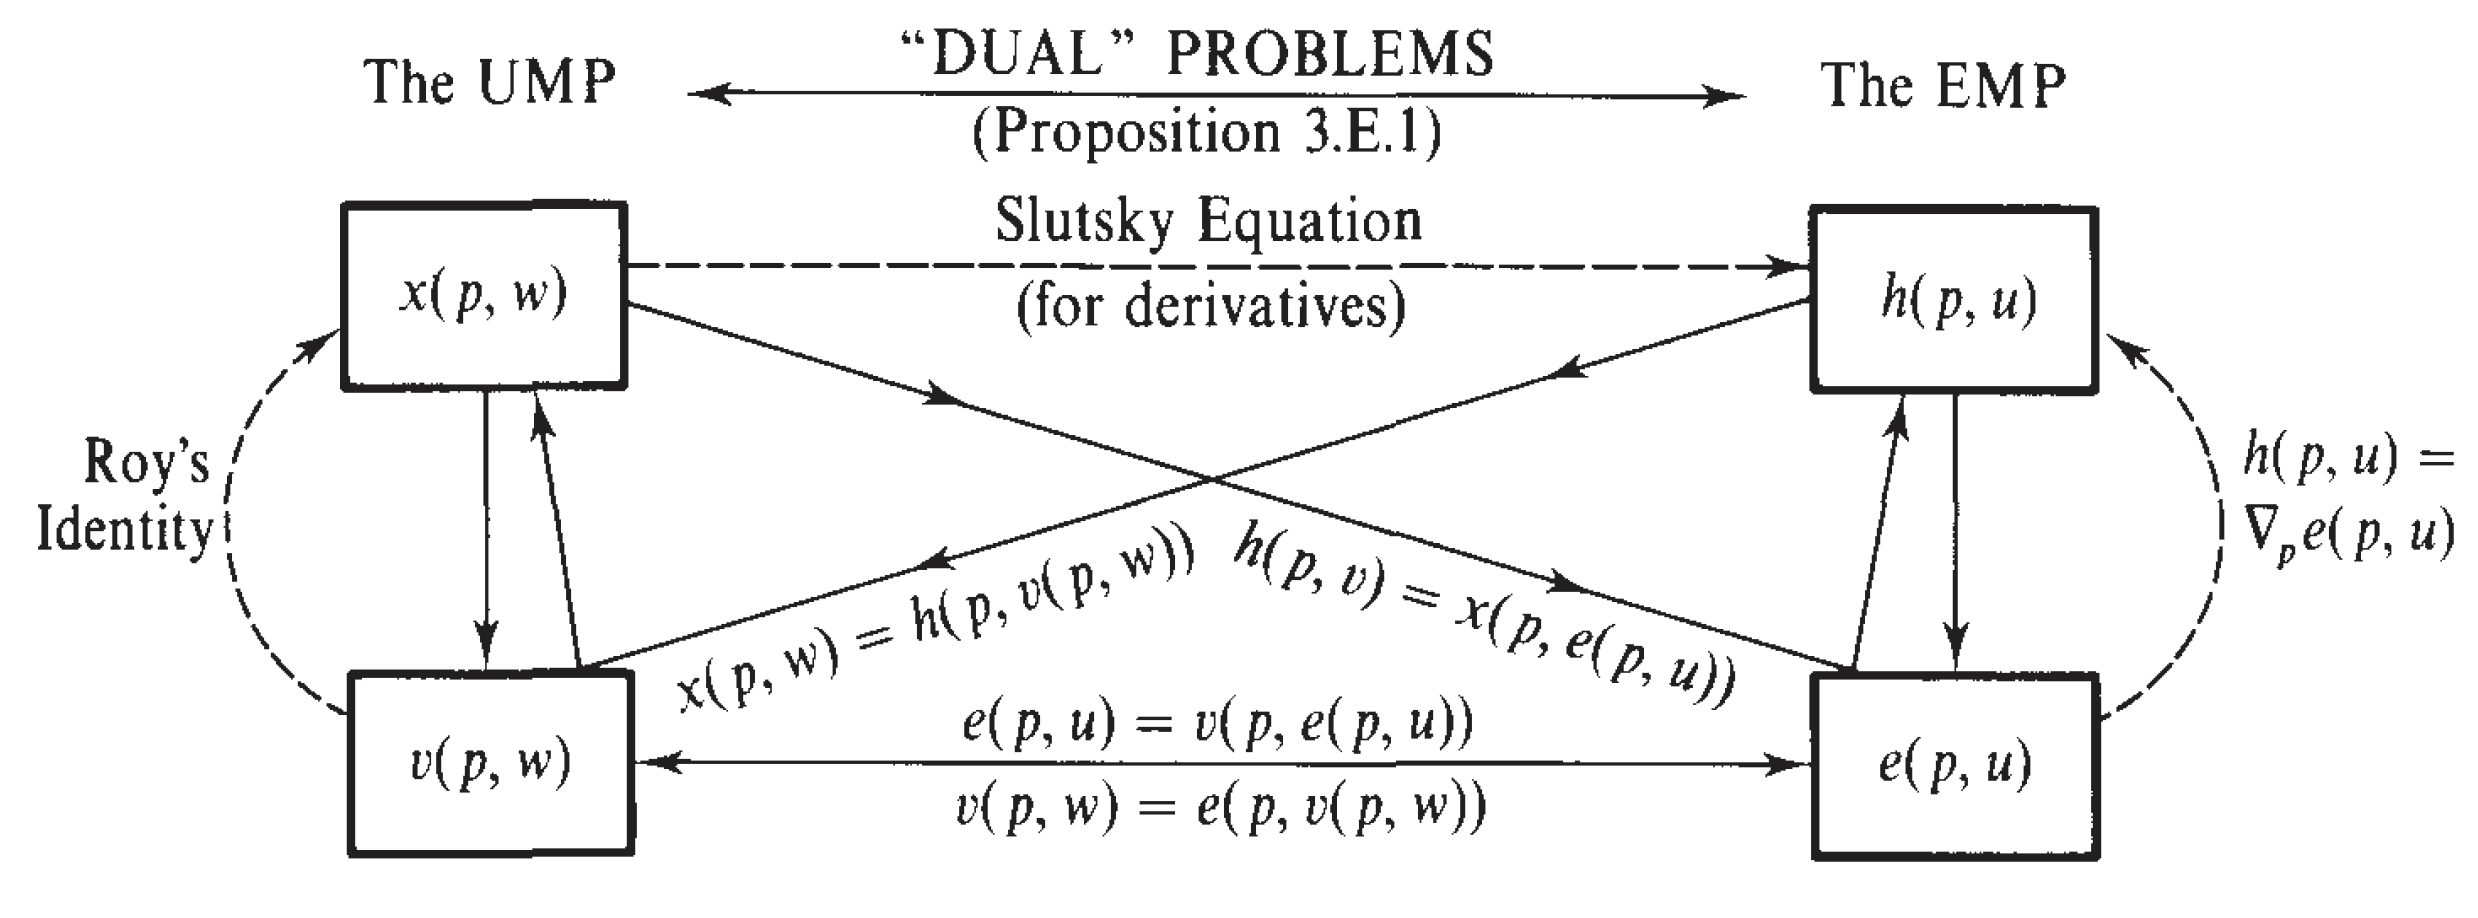
\includegraphics[width=1.0\linewidth]{figures/duality}
 				\caption{Fig. 3.G.3 in Mas-Colell: A Summary}
 			\end{figure}
 		
 		\subsection{Integrability}
 			\par \hl{TODO: this subsection needs revision.}
 			\begin{remark}[the Central Question]
 				Given a continuously differentiable demand function $x(p, w)$ satisfying homogenous of degree zero, Walras' law, and possessing negative semidefinite substitution matrix $S(p, w)$, can we find preferences rationalizing $x(p,w)$.
 			\end{remark}
 			
 			\begin{proposition}
 				Suppose the demand $x(p, w)$ satisfying the weak axiom, homogeneity of degree zero and Walras' law, then it can be rationalized by preferences \ul{if and only if} it has a symmetric substitution matrix $S(p, w)$.
 			\end{proposition}
 			
 			\subsubsection{Recovering Preferences from the Expenditure Function}
 			
 			\paragraph{Construction}For each utility level $u$, we can construct a \textbf{at-least-as-good-as set} $V_u \subset \R^L$ such that \ul{$e(p, u)$ is the minimal expenditure required for the consumer to purchase a bundle in $V_u$ at all price $p \gg 0$}. That's $V_u$ satisfies
 			\begin{equation}
 				\forall p \gg 0,\ e(p, u) = \min_{x \geq 0} p \cdot x\ s.t.\ x \in V_u
 			\end{equation}
 			
 			\begin{proposition}[3.H.1]
 				Suppose that $e(p, u)$ is strictly increasing in $u$ and is continuous, increasing, homogeneous of degree one, concave, and differentiable in $p$. Then, for every utility level $u$, $e(p, u)$ is the expenditure associated with at-least-as-good-as set
 				\begin{equation}
 					V_{u}=\left\{x \in \mathbb{R}_{+}^{L} : p \cdot x \geq e(p, u) \text { for all } p \gg 0\right\}
 				\end{equation}
 				That is, $e(p, u) = \min\{p\cdot x: x \in V_u\}\ \forall p \gg 0$.
 			\end{proposition}
 			
 			\par Then, for each $u > u(0)$, we can construct such $V_u$ and define $\pref$ on $X = \R^L_+$ with $V_u$. That's, for a given $x \in \R^L_+$ such that $u(x) \leftarrow \overline{u}$, then for each $y \in \R^L_+$,
 			\begin{equation}
 				y \pref x \iff y \in V_{\overline{u}}
 			\end{equation}
 			
 			\subsubsection{Recovering the Expenditure Function from Demand}
 			\paragraph{Construction} Suppose $x(p, w)$ is known, and by Shephard's lemma, expenditure function $e(p, w)$ can be solved from the system of partial differential equations
 			\begin{equation}
 				\begin{array}{l}{\frac{\partial e(p)}{\partial p_{1}}=x_{1}(p, e(p))} \\ {\vdots} \\ {\frac{\partial e(p)}{\partial p_{L}}=x_{L}(p, e(p))}\end{array}
 			\end{equation}
 			and initial conditions.
 			
 			\begin{proposition}
 				The necessary and sufficient condition for the recovery of an underlying expenditure function is the symmetry and negative semi-definiteness of the Slutsky matrix.
 			\end{proposition}
 		
 		\subsection{Welfare Evaluation of Economic Changes}
 			\paragraph{Context}We assume that the consumer has a fixed wealth level $w > 0$ and that the price vector is initially $p^0$. We wish to evaluate the impact on the consumer's welfare of a change from $p^0$ to a new price vector $p^1$.
 			
 			\begin{definition}
 				\textbf{Money metric} indirect utility functions measure welfare change expressed in dollar units. A money metric can be formed at an \ul{arbitrary price vector} $\overline{p} \gg 0$, and the welfare change expressed in dollar units is
 				\begin{equation}
 					e\left(\overline{p}, v\left(p^{1}, w\right)\right)-e\left(\overline{p}, v\left(p^{0}, w\right)\right)
 				\end{equation}
 			\end{definition}
 			
 			\begin{definition}
 				Let $u^0 = v(p^0, w)$, $u^1 = v(p^1, w)$, and noting that $e(p^0, u^0) = e(p^1, u^1) = w$.
 				When $\overline{p} = p^0$, the money metric is called \textbf{equivalence variation}
 				\begin{equation}
 					EV \left(p^{0}, p^{1}, w\right)=e\left(p^{0}, u^{1}\right)-e\left(p^{0}, u^{0}\right)=e\left(p^{0}, u^{1}\right)-w
 				\end{equation}
 				when $\overline{p} = p^1$, then it is referred to as
 				\begin{equation}
 					CV\left(p^{0}, p^{1}, w\right)=e\left(p^{1}, u^{1}\right)-e\left(p^{1}, u^{0}\right)=w-e\left(p^{1}, u^{0}\right)
 				\end{equation}
 			\end{definition}
 			
 			\begin{remark}[Interpretation of EV]
 				The equivalent variation can be thought of as the dollar amount that the consumer would be indifferent about accepting in lieu of the price change; that is, it is the change in her wealth that would be equivalent to the price change in terms of its welfare impact (so it is negative if the price change would make the consumer worse off). Therefore,
 				\begin{equation}
 					v(p^0, w+EV) = u^1
 				\end{equation}
 			\end{remark}
 			
 			\begin{remark}[interpretation of CV]
 				The compensating variation, on the other hand, measures the net revenue of a planner who must compensate the consumer for the price change after it occurs, bringing her back to her original utility level $u^0$ (Hence, the compensating variation is negative if the planner would have to pay the consumer a positive level of compensation because the price change makes her worse off.)
 				\begin{equation}
 					v\left(p^{1}, w-C V\right)=u^{0}
 				\end{equation}
 			\end{remark}
 			
 			\begin{proposition}
 				Suppose $p_1$ changes from $p_1^0$ to $p_1^1$, and $p^0_\ell = p^1_\ell = \overline{p}_\ell\ \forall \ell \neq 1$,
 				\begin{align}
 					EV\left(p^{0}, p^{1}, w\right) &=e\left(p^{0}, u^{1}\right)-w \\ 
 					&=e\left(p^{0}, u^{1}\right)-e\left(p^{1}, u^{1}\right) \\
 					&=\int_{p_{1}^{1}}^{p_{1}^{0}} h_{1}\left(p_{1}, \overline{p}_{-1}, u^{1}\right) d p_{1}
 				\end{align}
 				Similarly
 				\begin{align}
	 				CV\left(p^{0}, p^{1}, w\right) &= w - e(p^1, u^0) \\
	 				&= e(p^0, u^0) - e(p^1, u^0) \\
	 				&=\int_{p_{1}}^{p_{1}^{\circ}} h_{1}\left(p_{1}, \overline{p}_{-1}, u^{0}\right) d p_{1}
 				\end{align}
 			\end{proposition}
 			
 			\begin{remark}
 				However, if there is no wealth effect for good 1 (e.g., if the underlying preferences are quasilinear with respect to some good $\ell \neq 1$), the CV and EV measures are the same.
 			\end{remark}
 			
 			\begin{definition}
 				The value of area lying between $p_0^1$ and $p_1^1$ to the left of the market (Walrasian) demand curve for good 1, $\int_{p_1^1}^{p_1^0} x_1(p_1, \overline{p}_{-1}, w)\ dp_1$, measures the change in \textbf{Marshallian consumer surplus}. Such welfare measure is a special case of money metric when the wealth effects are absent.
 			\end{definition}
 			
 			\begin{definition}
 				Suppose the government imposes commodity tax of $t$ for each unit of good 1, let $T$ denote the amount of tax collected, then the \textbf{deadweight loss of commodity taxation} is 
 				\begin{align}
 					(-T)-E V\left(p^{0}, p^{1}, w\right) &=e\left(p^{1}, u^{1}\right)-e\left(p^{0}, u^{1}\right)-T \\
 					&=\int_{p_{1}^{0}}^{p_{1}^{0}+t} h_{1}\left(p_{1}, \overline{p}_{-1}, u^{1}\right) d p_{1}-t h_{1}\left(p_{1}^{0}+t, \overline{p}_{-1}, u^{1}\right) \\
 					&=\int_{p_{1}^{0}}^{p_{1}^{0}+t}\left[h_{1}\left(p_{1}, \overline{p}_{-1}, u^{1}\right)-h_{1}\left(p_{1}^{0}+t, \overline{p}_{-1}, u^{1}\right)\right] d p_{1}
 				\end{align}
 				It measures the extra amount by which the consumer is made worse off by commodity taxation above what is necessary to raise the same revenue through a lump-sum tax.
 			\end{definition}
 			
 			\subsubsection{Welfare Analysis with Partial Information}
 			
 			\begin{proposition}[3.I.1]
 				Suppose that the consumer has a locally nonsatiated rational preference relation $\pref$. If $(p^1-p^0) \cdot x^0 < 0$, then the consumer is strictly better off under price-wealth situation $(p^1, w)$ than $(p^0, w)$.
 			\end{proposition}
 			
 			\begin{proof}
 				By Walras' law, $p^0 \cdot x^0 = w$. Therefore, $x^0 \in B_{p_1, w}^{int}$. Because $x^0$ is in the interior of budget set, so $x^0 \neq x^1$ by local nonsatiation. As a result, $x^1 \succ^* x^0$ is revealed.
 			\end{proof}
 			
 			\begin{proposition}[3.I.2]
 				Suppose that the consumer has a differentiable expenditure function. then if $\left(p^{1}-p^{0}\right) \cdot x^{0}>0$, there is a sufficiently small $\overline{\alpha} \in (0, 1)$ such that for all $\alpha < \overline{\alpha}$, we have $\left(p^{1}-p^{0}\right) \cdot x^{0}>0$, and so the consumer is strictly better off under price-wealth situation $(p^0, w)$ than under $\left((1-\alpha) p^{0}+\alpha p^{1}, w\right)$
 			\end{proposition}
 			
 			\begin{definition}
 				The \textbf{area variation} measure (AV) provides an estimate of welfare change when only Walrasian demand is observable
 				\begin{equation}
 					A V\left(p^{0}, p^{1}, w\right)=\int_{p_{1}^{1}}^{p_{1}^{0}} x_{1}\left(p_{1}, \overline{p}_{-1}, w\right) d p_{1}
 				\end{equation}
 			\end{definition}
 			
 			\begin{remark}
 				When there are no wealth effects, $AV=EV=CV$.
 			\end{remark}
 			
 			\begin{remark}
 				Marshall argued that if a good is just one commodity among many, then because one extra unit of wealth will spread itself around, the wealth effect for the commodity is bound to be small; therefore, no significant errors will be made by evaluating the welfare effects of price changes for that good using the area measure.
 			\end{remark}
 			
 			\begin{remark}
 				So when $\Delta p$ is small, the error involved using the area variation measure becomes small as a fraction fo the true welfare change, and therefore, can be used as an accurate approximation of the actual welfare change.
 			\end{remark}
 			
 		\subsection{The Strong Axiom of Revealed Preference}
 			\begin{definition}[3.J.1]
 				The market demand function $x(p, w)$ satisfies the \textbf{strong axiom of revealed preference} (the SA) if for any sequence
 				\begin{equation}
 					\left(p^{1}, w^{1}\right), \ldots,\left(p^{N}, w^{N}\right)
 				\end{equation}
 				with $x\left(p^{n+1}, w^{n+1}\right) \neq x\left(p^{n}, w^{n}\right)$ for all $n \leq N-1$, we have 
 				\begin{equation}
 					\underbrace{p^{n} \cdot x\left(p^{n+1}, w^{n+1}\right) \leq w^{n}}_{x^n \succ^* x^{n+1} \tx{ revealed}}
 					\ \forall n \leq N - 1
 					\implies p^{N} \cdot x\left(p^1, w^1\right)>w^{N}
 				\end{equation}
 			\end{definition}
 			
 			\begin{proposition}[3.J.1]
 				If the Walrasian demand function $x(p, w)$ satisfies the strong axiom of revealed preference then there is a rational preference relation $\pref$ that rationalizes $x(p, w)$, that is, such that for all $(p, w)$, 
 				\begin{equation}
 					x(p, w) \succ y\ \forall y \in B_{p, w}\ s.t.\ y \neq x(p, w)
 				\end{equation}
 			\end{proposition}
 			
			\begin{proposition}[1.D.2 (\hl{WARP $\to$ Rational})]
				If $(\mathscr{B}, C(\cdot))$ is a choice structure such that
				\begin{enumerate}[(i)]
					\item The weak axiom is satisfied;
					\item $\mathscr{B}$ includes all subsets of $X$ up to three elements.
				\end{enumerate}
				Then there is a rational preference relation $\pref$ that rationalizes $C(\cdot)$ relative to $\mathscr{B}$.
			\end{proposition}
 			
 			\begin{remark}
 				Proposition 3.J.1 tells us that a choice-based theory of demand founded on the strong axiom is essentially equivalent to the preference-based theory of demand presented in this chapter.
 			\end{remark}
\end{document}



















































